\documentclass{scrartcl}
\usepackage{polyglossia}
\setdefaultlanguage{english}
\usepackage{xltxtra}
\setmainfont[Mapping=tex-text]{Junicode}
\newfontfamily{\avestan}[Scale=0.9]{Junicode}
\usepackage[letterpaper,margin=1in,includehead]{geometry}
\usepackage[object=vectorian]{pgfornament}
% MISC packages
\usepackage{hanging,verbatim,fancyhdr,xcolor,calc,multirow,longtable}
\usepackage[colorlinks=true, linkcolor=lightgray, urlcolor=lightgray, citecolor=lightgray]{hyperref}
\hypersetup{% 
pdftitle={Curriculum Vitae},%
pdfauthor={Suhas Mahesh}}
  \definecolor{gray}{HTML}{4D4D4D}
  \definecolor{white}{RGB}{255,255,255}
  \definecolor{lightgray}{RGB}{128,128,128}
\pagestyle{fancy}
  \fancyhf{}
  %\cfoot{Ollett CV\ \ {\footnotesize\fontspec{Printers Ornaments One}{\textcolor{gray}e}}\ \ \thepage}
  \renewcommand{\headrulewidth}{0pt}
\frenchspacing
\pagestyle{fancy}
\begin{document}
\setlength{\parindent}{0pt}

\newcommand{\whitelink}[2]{\href{#1}{\color{white}#2}}
\newcommand{\bluelink}[2]{\href{#1}{\color{blue}#2}}

\newcommand{\sectionline}{%
  \begin{center}
  {
    \resizebox{0.8\linewidth}{2ex}
    {{%
    {\color{gray}\begin{tikzpicture}
    \node  (C) at (0,0) {};
    \node (D) at (9,0) {};
    \path (C) to [ornament=88] (D);
    \end{tikzpicture}}}}}%
    \end{center}\bigskip
  }
  
% 
\definecolor{fillcolor}{RGB}{9,97,146}



\begin{tikzpicture}[remember picture,overlay]

% The clip x-shift has been set manually. You need to re-adjust. To adjust, replace \clip by \draw (with same arguments) so you can see the box.
\clip [rounded corners=10mm] ([xshift =-10.55cm,yshift=-0.25cm]current page.north) rectangle ++(\paperwidth-0.5cm,-4.5cm);

  % Existing nodes
  \node [rounded corners=10mm, rectangle, draw=fillcolor, fill=fillcolor, anchor=north, minimum width=\paperwidth-0.5cm, minimum height=4.5cm] (box) at ([yshift=-0.25cm]current page.north){};
  
 
  \node [anchor=center] (name) at ([yshift=0.3cm]box) {%
    \fontsize{40pt}{72pt}\color{white}%
    \textsc{Suhas Mahesh{\kern0pt}}
  };
	
  % New node for Schrodinger's Equation
  \node [rotate=45, anchor=south east, opacity=0.2] at ([yshift=5cm, xshift=-2cm]box.south east) {
    \color{white} % Set the color of the equation
    \fontsize{30pt}{36pt}\selectfont % Set the font size
    $i\hbar\frac{\partial}{\partial t}\Psi(\mathbf{r},t) = \hat{H}\Psi(\mathbf{r},t)$
  };
  
  % New node for the image
  \node [anchor=south west, opacity=0.5] at ([yshift=-1cm, xshift=-3cm]box.south west) {
    
\includegraphics[width=6cm]{img/organicmol.png} % Adjust the width as necessary
  };
  
    % New node for the image
  \node [anchor=south west, opacity=0.5] at ([yshift=-3cm, xshift=17cm]box.south west) {
    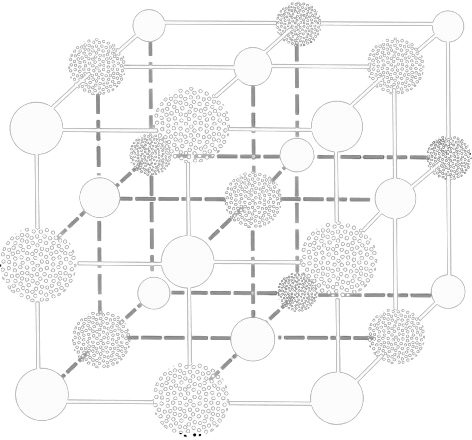
\includegraphics[width=6cm]{img/crystal.png} % Adjust the width as necessary
  };
  
      % New node for the image
  \node [anchor=south west, opacity=0.1] at ([yshift=-2cm, xshift=5cm]box.south west) {
    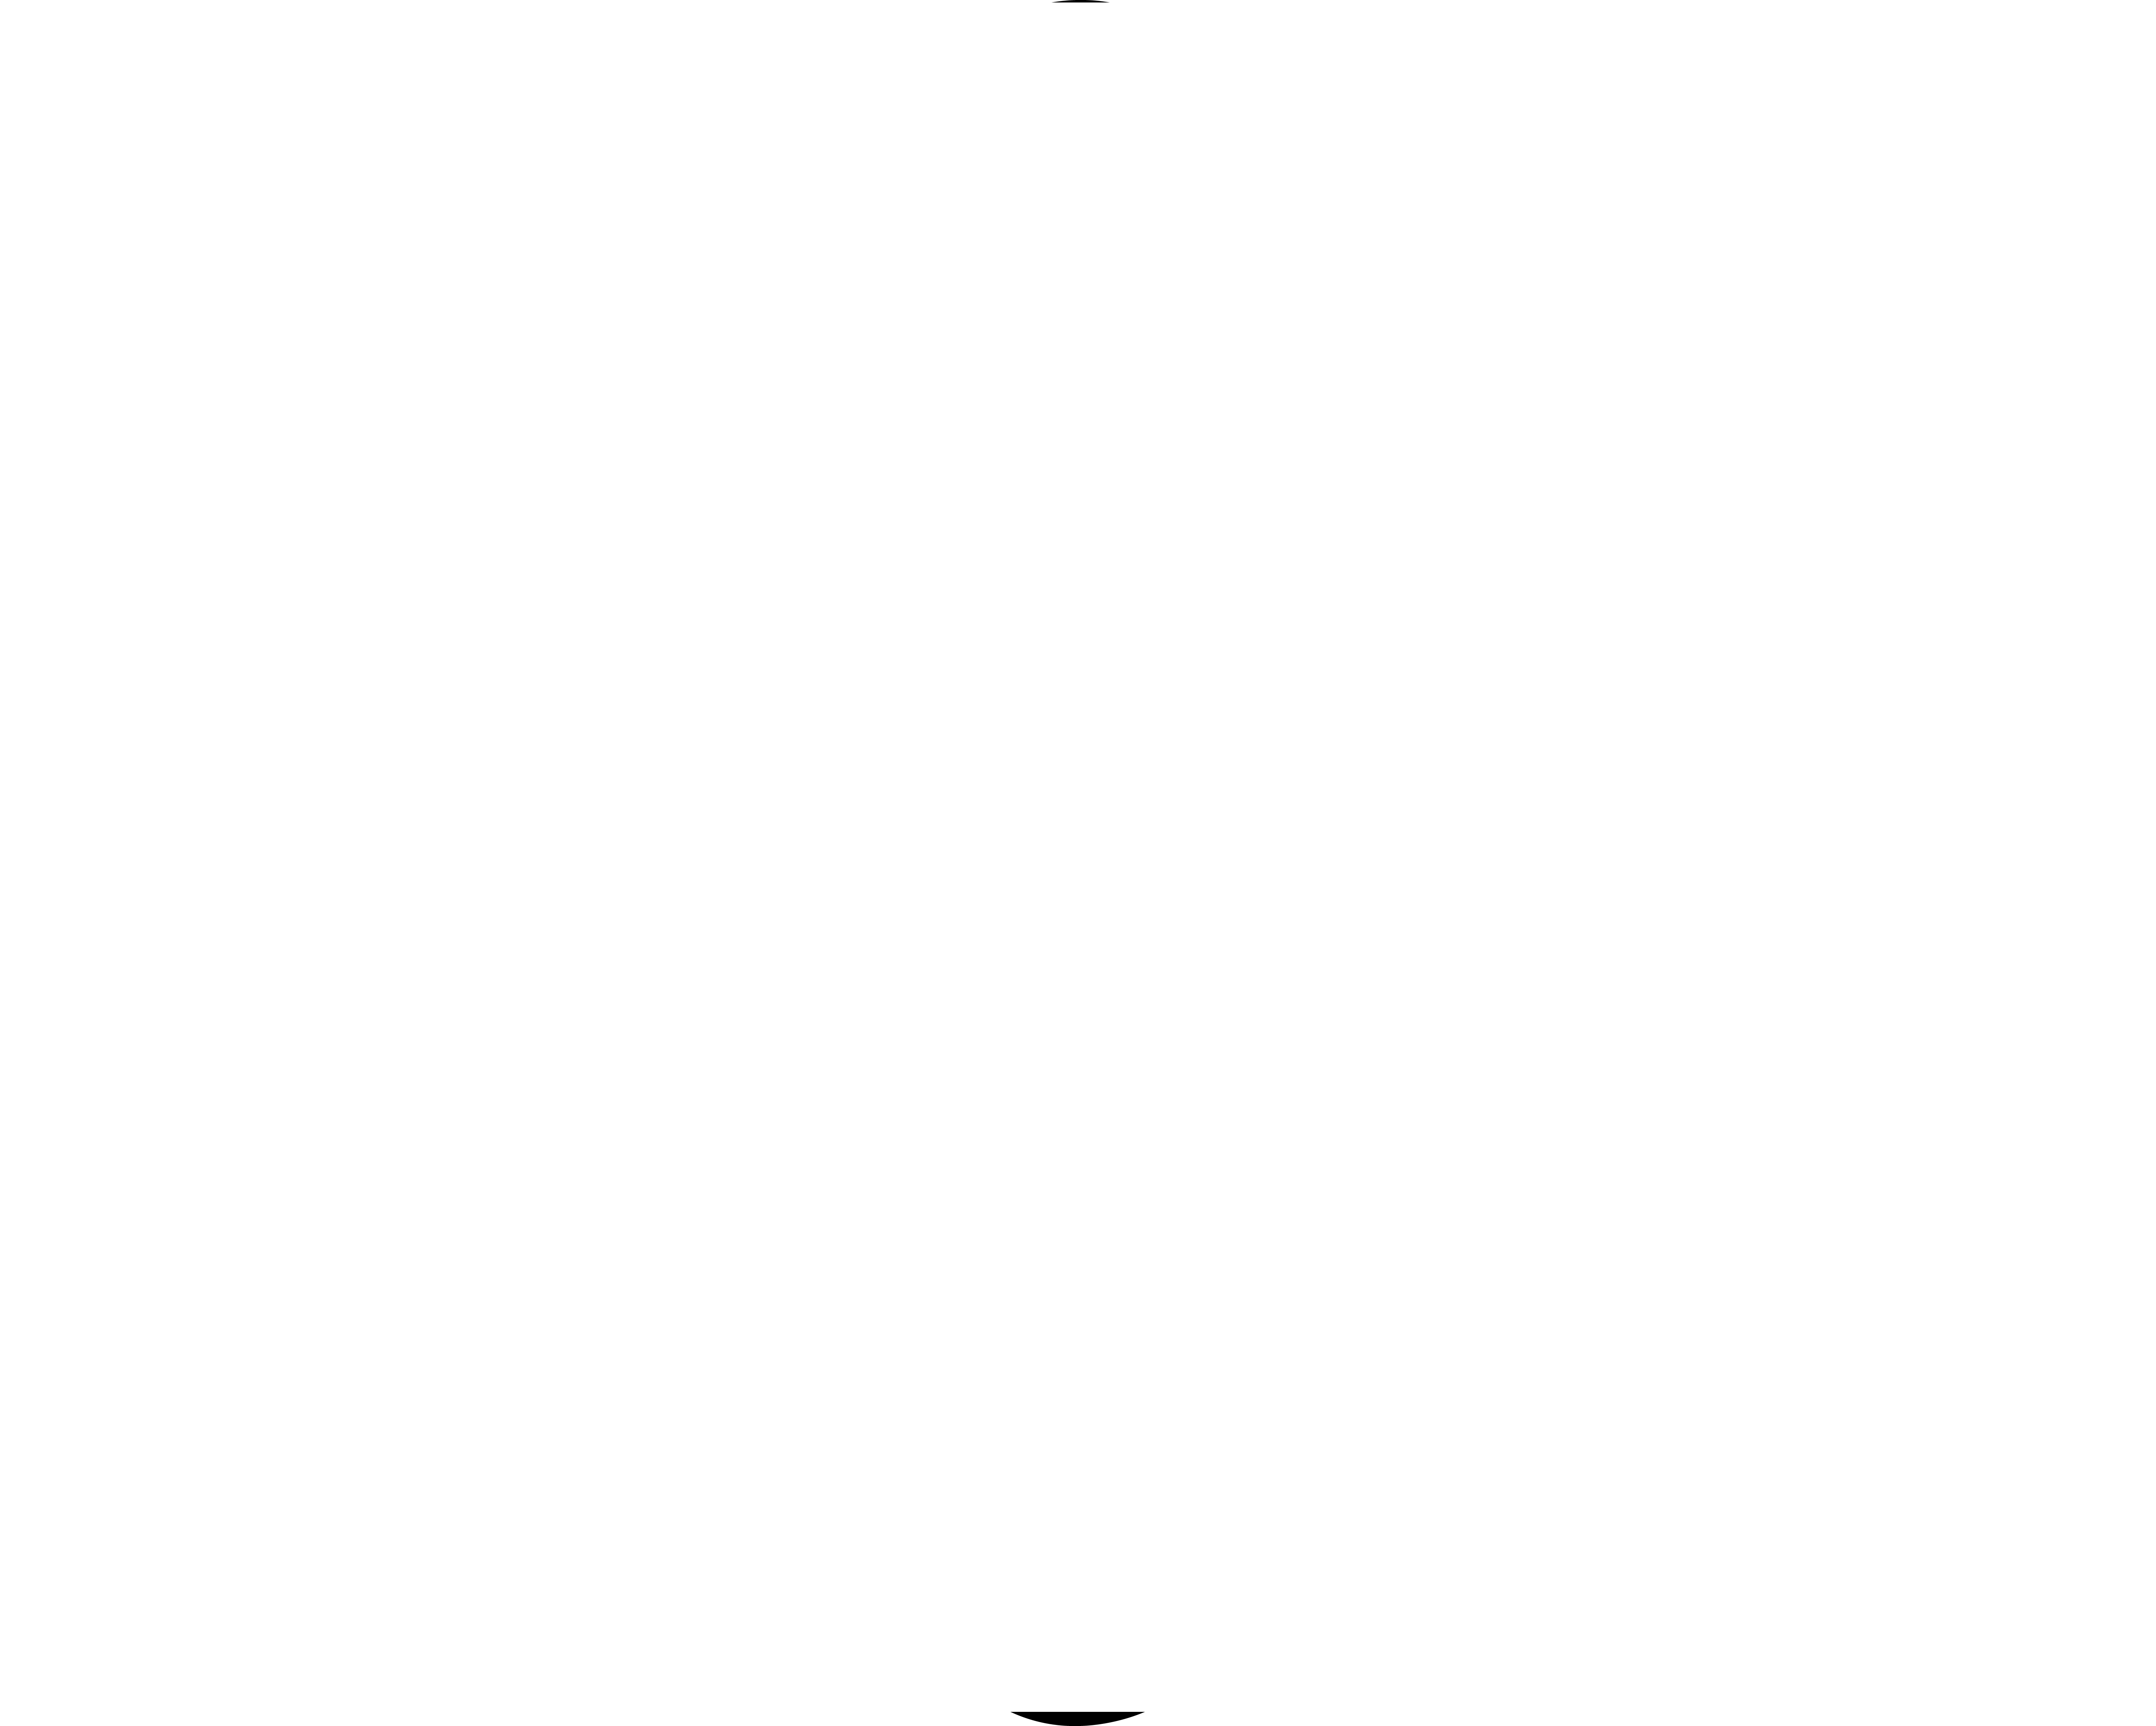
\includegraphics[width=6cm]{img/nn.png} % Adjust the width as necessary
  };
  
  \node [align=left, text width=10cm, rotate=20, anchor=south east, opacity=0.2] at ([yshift=5cm, xshift=-9cm]box.south east) {
   \color{white}
    \texttt{from pymatgen.core import *\\
            from pymatgen.io.vasp.sets import *\\
            from pymatgen import Lattice, Structure, Molecule\\
            from pymatgen.io.vasp.sets import MPRelaxSet}
  };
  
\end{tikzpicture}


\vspace{0.8cm}
\newcommand{\pgfdot}{\hspace{1em}\tikz\draw[fill=black] (0,0) circle (.5ex);\hspace{1em}}


\vspace{-2.0cm}
\begin{center} 
{{\small 
\begin{tabular}{ccccccc}
  \multirow{2}{*}{\color{white}\whitelink{https://twitter.com/suhasm}{Twitter}} & \multirow{2}{*}{\color{white}} & 
  \multirow{2}{*}{\color{white}\whitelink{https://www.linkedin.com/in/suhas-mahesh-0b366a71/}{LinkedIn}} & \multirow{2}{*}{\color{white}} &  \multirow{2}{*}{\color{white}\whitelink{http://www.suhasmahesh.com}{suhasmahesh.com}} &
  \multirow{2}{*}{\color{white}} & \multirow{2}{*}{\color{white}\whitelink{mailto:suhas.mahesh@utoronto.ca}{suhas.mahesh@utoronto.ca}}
\end{tabular} }} \end{center}\par\vspace{1cm}

Lorem ipsum dolor sit amet, consectetur adipiscing elit, sed do eiusmod tempor incididunt ut labore et dolore magna aliqua. Ut enim ad minim veniam, quis nostrud exercitation ullamco laboris nisi ut aliquip ex ea commodo consequat. Duis aute irure dolor in reprehenderit in voluptate velit esse cillum dolore eu fugiat nulla pariatur. Excepteur sint occaecat cupidatat non proident, sunt in culpa qui officia deserunt mollit anim id est laborum \vspace{1cm}

\newcommand{\secttitle}[1]{{{\Large\textbf{#1}}}\par\medskip}
\newcommand{\sectsubtitle}[1]{{{\large\textbf{#1}}}\par\medskip}

\setlength{\tabcolsep}{0pt}
\newenvironment{entrylist}{%
  \begin{longtable}{@{\extracolsep{\fill}}ll}
}{%
  \end{longtable}
}
\newcommand{\entry}[4]{%
  {\addfontfeature{Color=gray} #1}&\parbox[t]{0.8\textwidth}{%
    \textbf{#2}\hfill #3\\ #4\vspace{\parsep}%
  }\\}
\newcommand{\refentry}[3]{%
  {\addfontfeature{Color=gray} #1}&\parbox[t]{0.8\textwidth}{%
    \raggedright#2\\ {{\raggedright\small #3}}\vspace{\parsep}%
  }\\}
\newcommand{\singleentry}[2]{%
  {\addfontfeature{Color=gray} #1}&\parbox[t]{0.8\textwidth}{%
    #2\vspace{\parsep}%
  }\\}
\newcommand{\splitentry}[4]{%
  {\addfontfeature{Color=gray} #1}&\parbox[t]{0.8\textwidth}{%
    \raggedright #2\hfill #3\\ \raggedright\small #4\vspace{\parsep}%
  }\\}


\raggedright

\secttitle{Employment}
\begin{entrylist}
\entry
{Sep 2021–}
{Schmidt Science Fellow \textnormal{\href{https://schmidtsciencefellows.org/fellow/suhas-mahesh/}{link}}}
{University of Toronto}
{Department of Electrical \& Computer Engineering}
\end{entrylist}

\secttitle{Education}

\begin{entrylist}
\entry
{2016--2021}
{Doctor of Philosophy in Condensed Matter Physics}
{University of Oxford}
{Rhodes Scholarship \href{https://www.rhodeshouse.ox.ac.uk/scholars/rhodes-scholars-class-of-2016/suhas-mahesh/}{link}\\
Supervisor: Prof. Henry Snaith, FRS \href{https://scholar.google.com/citations?user=I2D3pUMAAAAJ&hl=en}{link}\\
\emph{Optical and Electronic Studies of New Materials for Multijunction Photovoltaics }\href{http://dx.doi.org/10.5287/bodleian:mNArOK77N}{link}\\
Thesis award (2021) from MPLS Division, University of Oxford \\
}

\entry
{2012--2016}
{Bachelor of Science in Physics}
{Indian Institute of Science}
{With highest honors}

\entry
{2016}
{Research Intern}
{Italian Institute of Technology}
{Inkjet Processed Semiconductors \href{https://scholar.google.it/citations?user=f3suRUkAAAAJ&hl=en}{link}}

\entry
{2015}
{Research Intern}
{University of Groningen, Netherlands}
{Carbon Nanotube based FETs \href{https://scholar.google.com/citations?user=Cw22GB8AAAAJ&hl=en}{link}}
\end{entrylist}

\secttitle{Published Articles and Book Chapters}\bigskip
\sectsubtitle{Please see my \bluelink{https://scholar.google.com/citations?user=Y5ReiQsAAAAJ&hl=en}{Google Scholar}} A partial list of publications is provided at the end of this CV. \bigskip

\secttitle{Patents}

\begin{entrylist}
\splitentry
{Pending}{Snaith, H. J and Mahesh, S. \textbf{Multi-Junction Optoelectronic Device Comprising Device Interlayer}, International Application Number: PCT/GB2019/053550 \href{https://patents.google.com/patent/WO2020120991A1/}{link} }{}

\end{entrylist} 


\secttitle{Grants, Fellowships and Prizes}

\begin{entrylist}
\refentry
{2024}{Catalyst Interdisciplinary Grant (\$10,000) (co-PI with Sebastian Musslick) \href{https://schmidtsciencefellows.org/news/2023-catalyst-grants-awardees/}{link} }{}
\refentry
{2023}{Software engineering grant (1 FTE-year), Virtual Institute for Scientific Software \href{https://www.schmidtfutures.com/our-work/virtual-institute-for-scientific-software/}{link} }{}
\refentry
{2023}{Acceleration Consortium Fellowship (\$110,000) \href{https://acceleration.utoronto.ca/}{link} }{}
\refentry
{2022}{Optoelectronics Materials Discovery Grant, Schmidt Futures (\$42,000) \href{https://www.schmidtfutures.com/}{link} }{}
\refentry
{2021}{Schmidt Science Fellowship (\$200,000) \href{https://schmidtsciencefellows.org/}{link} }{}
\refentry
{2016}{Rhodes Scholarship (\$150,000)}{}
\refentry
{2019}{Best Early Career Presentation, SUNRISE Solar Symposium (London)}{}
\refentry
{2019}{Best Early Career Presentation (\$110,000)}{}
\refentry
{2016}{Best Speaker Award (\$110,000)}{}
\end{entrylist} 

\secttitle{Recent Invited Talks}

\begin{entrylist}

\splitentry
{2023}
{ML-guided Discovery of Two-Dimensional Perovskites (invited)}
{Synthace}{}

\splitentry
{2023}
{Beating the Negative Data Problem in Materials Science (invited)}
{Rhodes Trust}{}

\splitentry
{2022}
{Thermodynamics of Optoelectronic Devices (invited)}
{University of Oxford}{}

\splitentry
{2021}
{Computational Modelling of Solar Absorbers (invited)}
{IISER Berhampur}{}

\splitentry
{2021}
{Spatial Inhomogeneities in Perovskite Photovoltaics (invited)}
{SUNRISE Symposium}{}

\splitentry
{2020}
{Origin of Phase Instabilities in Perovskite Semiconductors (invited)}
{Oxford PV}{}




\end{entrylist}


\secttitle{Teaching Experience}

Semiconductor Devices, Organic Electronics , Solar Cell Thermodynamics, Condensed Matter Physics (TA), Analogue Electronics (TA). More detailed teaching history can be provided upon request.\bigskip

\secttitle{Outreach and Community}

\begin{entrylist}

\splitentry
{2023}
{Selector for Rhodes Scholarship}
{Rhodes Trust}{}

\splitentry
{2021}
{Selector for the RISE Award \href{https://www.risefortheworld.org/}{link}}
{RISE}{}

\splitentry
{2019}
{Conference for Undergraduate Women in Physics (co-organiser)}
{Institute of Physics}{}

\splitentry
{2019}
{Stargazing Science Festival (outreach exhibit) \href{https://web.archive.org/web/20230402133900/https://www.physics.ox.ac.uk/news/stargazing-oxfordhome}{link}}
{University of Oxford}{}

\splitentry
{2018}
{Oxford Science Festival (outreach exhibit) \href{https://web.archive.org/web/20230208050049/https://scienceoxford.com/events/oxfordshire-science-festival/}{link}}
{University of Oxford}{}

\splitentry
{2014-16}
{Head of Scholarships, Notebook Drive \href{https://web.archive.org/web/20230126231829/https://iisc.ac.in/outreach/activities/notebook-drive/}{link}}
{Notebook Drive}{Notebook Drive is an NGO working to improve access to primary education in rural India.}

\end{entrylist}

\secttitle{Other Interests}

\begin{entrylist}

\splitentry
{2023–}
{Co-creator of ambuda.org \href{https://www.ambuda.org}{link}}
{}{Breakthrough digital library of Sanskrit with intelligent ML-based tools}

\splitentry
{2024}
{\emph{How to Love in Sanskrit} (HarperCollins; co-authored with Anusha Rao)}
{}{Compendium of 3000 years of Sanskrit wisdom on love, in English translation}

\end{entrylist}




\vfill


\end{document}
